\documentclass[11pt,a4paper]{article}

% --- Encoding, language, and margins ---
\usepackage[utf8]{inputenc}
\usepackage[T1]{fontenc}
\usepackage[english]{babel}
\usepackage{geometry}
\geometry{margin=2.5cm}

% --- Math and layout ---
\usepackage{amsmath, amssymb, amsfonts}
\usepackage{graphicx}
\usepackage{float}
\usepackage{fancyhdr}
\usepackage{lastpage}
\usepackage{setspace}
\usepackage{xcolor}
\usepackage{hyperref}
\usepackage{subcaption}
\usepackage{enumitem}
\usepackage[ruled,vlined,linesnumbered]{algorithm2e}
\usepackage{boxedminipage}
\usepackage{amsthm}
\usepackage{tikz}
\usepackage{tikz-cd}
\usepackage{booktabs}

% Figures are found whether the report is compiled from report/ or from the repo root.
\graphicspath{{./}{report/}{../figures/analysis/}{figures/analysis/}}

% --- Spacing and style ---
\onehalfspacing
\setlength{\parskip}{0.5em}
\setlength{\parindent}{0pt}

% --- Headers and footers ---
\setlength{\headheight}{14pt}
\pagestyle{fancy}
\fancyhf{}
\lhead{\textbf{SF2956: Topological Data Analysis}}
\rhead{Project: Neurons differentiation --- November 2026}
\cfoot{\thepage/\pageref{LastPage}}
% Front matter (table of contents): roman page number only, no "/total".
\fancypagestyle{frontmatter}{%
    \fancyhf{}%
    \lhead{\textbf{SF2956: Topological Data Analysis}}%
    \rhead{Project: Neurons differentiation --- November 2026}%
    \cfoot{\thepage}%
}

% --- Discreet hyperlinks ---
\hypersetup{
    colorlinks = true,
    linkcolor = blue!60!black,
    urlcolor  = blue!70!black
}

% --- Document information ---
\title{Project: Neurons differentiation}
\author{Ahou Lucas\\Powierski Maxim\\Peduzzi Lionel}
\date{November 2026}

\begin{document}

% =========================================================
%                       FRONT PAGE
% =========================================================
\begin{titlepage}
    \thispagestyle{empty}
    \centering
    \vspace*{2cm}

    {\large \textsc{KTH Royal Institute of Technology}\par}
    \vspace{0.5cm}
    {\large SF2956: Topological Data Analysis\par}

    \vspace{2.5cm}
    \hrule height 1pt
    \vspace{0.8cm}
    {\Huge \bfseries Project:\\[0.3em] Neurons differentiation\par}
    \vspace{0.8cm}
    \hrule height 1pt

    \vspace{3cm}
    {\large \textbf{Authors}\par}
    \vspace{0.4cm}
    {\large
    Ahou Lucas\\[0.2em]
    Powierski Maxim\\[0.2em]
    Peduzzi Lionel\par}

    \vfill
    {\large November 2026\par}
    \vspace{1cm}
\end{titlepage}

% =========================================================
%                   TABLE OF CONTENTS
% =========================================================
\pagenumbering{roman}
\setcounter{page}{1}
\pagestyle{frontmatter}
\setcounter{tocdepth}{2}  % sections and subsections only, so the contents fit on one page
\tableofcontents
\clearpage
\pagestyle{fancy}

\pagenumbering{arabic}
\setcounter{page}{1}

% =========================================================
%                         CONTENT
% =========================================================
\section{Subject introduction}
\label{sec:intro}

Neurons communicate with short electrical pulses called \textbf{spikes}. When we record a neuron, we get a list of the times when it fired. This list is called a \textbf{spike train}. The shape of a single spike carries almost no information: all spikes look the same. The information is in the timing of the spikes.

In the retina, there are many different types of neurons. For example, in the mouse there are more than 30 types of retinal ganglion cells. Each type reacts to a different feature of the image: some react when the light turns on, some when it turns off, some to motion, and so on. Two neurons that see the same image can therefore produce very different spike trains. But two recordings of the same neuron should look similar, even if they are not exactly the same, because neurons are noisy.

This leads to the question of our project:
\begin{center}
    \textit{Given a single spike train, can we tell which neuron it comes from?}
\end{center}
In other words, we want to know if each neuron has its own ``signature'' in its spike trains. If this signature exists, it should also help to separate neurons into groups, and maybe later into cell types.

To study this question, we need a good way to compare spike trains. This is not easy. A spike train is not a vector of fixed size: two trials can have a different number of spikes. Also, small shifts in time should only change the distance a little. Classical tools exist, like comparing histograms of interspike intervals or counting spikes in time windows. In this project, we try to use \textbf{topological data analysis} (TDA) instead. The idea is to transform each spike train into a geometric object, a point cloud. Then we compute its homology and use the stable rank (see Section~\ref{sec:math}) to turn it into a function. These functions are easy to compare, and the stable rank is stable: a small change in the spike train gives a small change in the function.

To test this, we need data where the same neuron is recorded many times under the same conditions. We use recordings of mouse retinal ganglion cells that see the same white noise movie repeated about 30 times (see Section~\ref{sec:data}). For each trial, we check if the closest spike trains come from the same neuron. We compare the TDA methods with simpler methods that do not use topology.

\section{Data set}
\label{sec:data}

\subsection{The experiment}
We use a public dataset from Karamanlis and Gollisch\footnote{D. Karamanlis and T. Gollisch (2021), \textit{Nonlinear spatial integration underlies the diversity of retinal ganglion cell responses to natural images}, J Neurosci 41:3479--3498. The data is available on the \href{https://gin.g-node.org/gollischlab/Karamanlis_Gollisch_2021_RGC_spiketrains_natural_image_encoding}{G-Node GIN platform}.}. In this experiment, the retina of a mouse was taken out and placed on a multielectrode array. This array has 252 electrodes. Each electrode records the electrical activity of the neurons that are close to it. The recorded neurons are retinal ganglion cells. These cells are the output neurons of the retina: they send the visual information to the brain.

During the recording, the retina was stimulated with light patterns shown on a small screen. A spike sorting algorithm was then used to find the spikes of each neuron in the electrode signals. The authors also gave a list of the ``good'' neurons, which are the ones that were sorted well. We only use these neurons. The full dataset contains 13 recording sessions.

\subsection{The stimulus}
The authors used many different stimuli. We only use one of them: the \textbf{frozen noise}. It is a white noise movie made of black and white squares. Each square is black or white at random, with probability $1/2$.

The stimulus alternates between two parts:
\begin{itemize}
    \item a \textit{running} part: 1500 frames of new random noise (about 50 seconds),
    \item a \textit{frozen} part: 300 frames of a fixed noise movie (about 10 seconds).
\end{itemize}
The frozen part is always the same movie. So each neuron sees exactly the same stimulus many times. We call each presentation of the frozen part a \textbf{trial}. This is useful for us: since the input is the same, the differences between neurons come from the neurons themselves and not from the stimulus.

\subsection{Building our dataset}
Only 9 of the 13 sessions contain the frozen noise stimulus, so we keep these 9 sessions. For each good neuron, we cut its spike train into trials. A trial starts at the beginning of a frozen part and lasts about 9.94 seconds. We shift the spike times so that each trial starts at time 0. Then we compute the interspike intervals (ISIs), which are the times between two consecutive spikes:
\[
    \text{ISI}_i = t_{i+1} - t_i .
\]
If a trial has less than 2 spikes, its list of ISIs is empty. We keep these trials anyway.

Our final dataset contains:
\begin{itemize}
    \item 850 neurons from 9 sessions,
    \item 30 trials per neuron in most sessions (31 and 34 in two sessions),
    \item 25\,873 spike trains in total (one per neuron and per trial).
\end{itemize}
The neurons fire at very different rates. The median firing rate is 5.7 Hz, and half of the neurons fire between 2.4 Hz and 14.2 Hz. 42 neurons fire less than 0.5 Hz, so they have very few ISIs. We do not have any labels for the cell types. We only know the identity of each neuron.

\subsection{First observations}
Figure~\ref{fig:raster} shows the spikes of one neuron for all its trials. We can see vertical lines: the neuron often fires at the same times in different trials. This means that the response is locked to the stimulus. To check this for all neurons, we computed the correlation between the firing rates of different trials. The median correlation is 0.16. When we shift the trials randomly in time, it drops to 0. So most neurons respond in a reliable way to the frozen noise.

We also noticed that the neurons fire a bit more at the end of the recording than at the beginning (about 93 spikes per trial in the first trials, against about 115 in the last ones). Some neurons are even almost silent during the first trials. We have to keep this in mind, because the trials are not perfectly identical.

\begin{figure}[H]
    \centering
    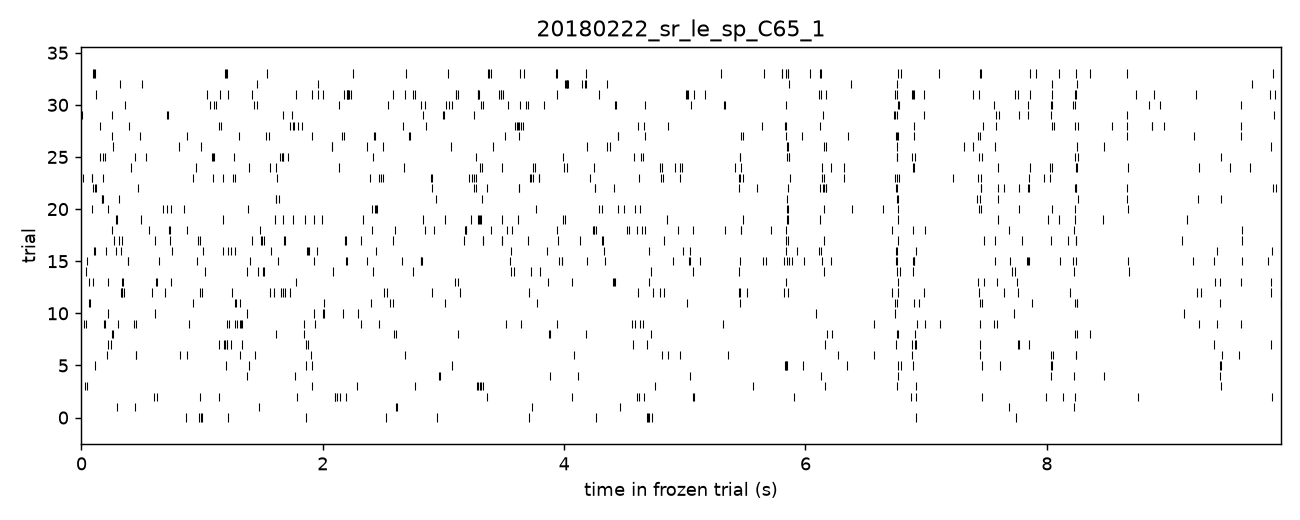
\includegraphics[width=0.95\linewidth]{raster_20180222_sr_le_sp_C65_1.png}
    \caption{Raster plot of one neuron (session 20180222\_sr\_le\_sp). Each line is one trial, and each tick is a spike.}
    \label{fig:raster}
\end{figure}

Figure~\ref{fig:isi_hist} shows the distribution of the ISIs for three neurons. We use a logarithmic scale, because the ISIs go from about 1 ms (inside a burst of spikes) to more than 1 second (pauses). The three distributions have different shapes. The blue and orange neurons have two peaks: very short ISIs of a few milliseconds (spikes inside a burst) and longer ISIs of about 0.1 to 0.2 seconds (between bursts). But the peaks are not at the same place and do not have the same height. The green neuron fires much faster, and most of its ISIs are shorter than 30 ms. This already suggests that the ISIs carry information about the identity of the neuron.

\begin{figure}[H]
    \centering
    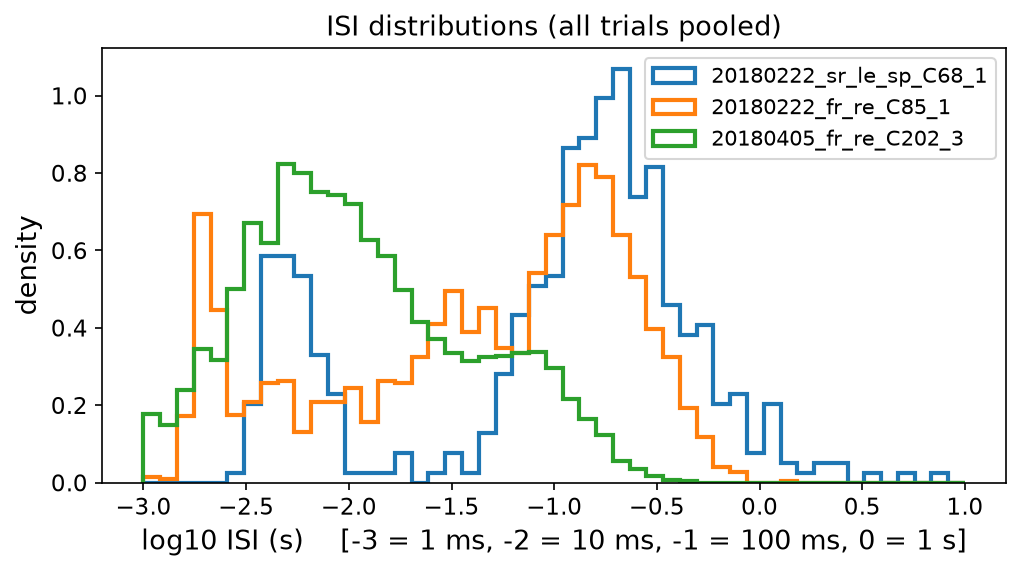
\includegraphics[width=0.65\linewidth]{explore_isi_hist.png}
    \caption{Distribution of $\log_{10}$ ISI for three neurons (all trials pooled).}
    \label{fig:isi_hist}
\end{figure}


\section{Mathematical background}
\label{sec:math}
Before using any methods to analyse the dataset, we will introduce the main ideas of the methods and the mathematical concepts needed to understand these methods.

\subsection{Framework}
The basic idea of the method is to transform any dataset into a mathematical object on which it is more convenient to perform statistical and ML analysis. More formally, our data sets are described by a metric space $(X,d)$ and we would like to map it to a piecewise constant function (PCF). This procedure tries to capture the structure (the invariants) of this dataset.

Here are two ways to describe the procedure of the method:

\textbf{First:}
\begin{enumerate}
    \item Choose an extension $\psi$ and create a dendrogram $D$ as the hierarchical clustering of $X$ with respect to $\psi$
    \item Choose a field K and create a tame vector space parametrized by $[0,\infty)$: $V=KD$
    \item Use the stable rank to transform the vector space into a PCF.
\end{enumerate}

\textbf{Second:}
\begin{enumerate}
    \item Create a simplicial complex from X through Vietoris-Rips: $S=VR_t(X)$
    \item Choose a field K and create the $n^{th}$ homology of $S$: $V=H_n(S,K)$
    \item Use the stable rank to get a PCF: $\widehat{rank}\,V(t)$
\end{enumerate}

The first procedure with a single linkage as an extension is equivalent to the second one with $n=0$. But, by increasing $n$, we can get a new family of methods that provide more information about the data set.


\subsection{Hierarchical clustering}
Clustering consists in grouping the points of a dataset $(X,d)$ so that points in the same group are close to each other.

Hierarchical clustering returns a family of nested partitions, from the finest one (every point alone) to the coarsest one (a single cluster).

To merge clusters, we need a notion of distance between clusters, not only between points.

\textbf{Definition:}
An \emph{extension} (or \emph{linkage}) $\psi$ transforms a distance $d$ between elements of $X$ into a distance $\psi d$ between non-empty subsets $A,B \subseteq X$, such that $\psi d(\{x\},\{y\}) = d(x,y)$ for all $x,y\in X$.

Here are two examples of extensions.
\begin{align*}
\psi_{\text{single}}(A,B) &= \min_{a\in A,\, b\in B} d(a,b), &
\psi_{\text{complete}}(A,B) &= \max_{a\in A,\, b\in B} d(a,b)
\end{align*}

\textbf{Algorithm:}
Given $(X,d)$ and an extension $\psi$:
\begin{enumerate}
    \item Start with the partition $P_0=\{\{x\} \mid x\in X\}$ and set $a_0=0$.
    \item For $k=0,\dots,N-2$: choose two distinct elements $A,B$ of $P_k$ that minimise $\psi d(A,B)$, set $a_{k+1}=\psi d(A,B)$ and
    \[
        P_{k+1} = \big(P_k \setminus \{A,B\}\big)\cup\{A\cup B\}.
    \]
\end{enumerate}
The output is the sequence of partitions $P_0, P_1, \dots, P_{N-1}=\{X\}$ and the sequence $a_0,\dots,a_{N-1}$.

Remark: If there exist several pairs $A,B$ of $P_k$ that minimise $\psi d(A,B)$, we can merge them at the same time to make the transformation independent of the order of the elements.


\subsection{Dendrograms}
The output of the hierarchical clustering is encoded by an object called a dendrogram.

\textbf{Definition:}
A \textbf{dendrogram} of $X$ is defined by associating to each value of $t \in [0,\infty)$ a partition $D_t$ of $X$. It must also contain the definition of the maps between partitions: $\forall t_1, t_2 \in [0,\infty) \, s.t. \, t_1<t_2: \exists D_{t_1<t_2}: D_{t_1} \rightarrow D_{t_2}$. And the following properties must be fulfilled:

$\forall t_1, t_2, t_3 \in [0,\infty) \, s.t. \, t_1<t_2<t_3:  D_{t_2<t_3} (D_{t_1<t_2}) = D_{t_1<t_3}$.

There must also exist a sequence of real numbers: $0=a_0<a_1<\dots<a_n$ such that the transition between $D_{t_1}$ and $D_{t_2}$ is an isomorphism if $t_1$ and $t_2$ belong to the same interval among $[a_0,a_1),[a_1,a_2),\dots,[a_n,\infty)$.

\textbf{Dendrogram as a graph:}
It can be represented by a graph where lines gather when the sets merge.

\begin{figure}[H]
    \centering
    \begin{tikzpicture}[x=1.1cm, y=0.75cm]
        % leaves a,b,c,d,e at x = 0,...,4 ; merge heights 1, 1.5, 2, 3.5
        \draw[->] (-0.8,0) -- (-0.8,4.6) node[above] {$t$};
        \foreach \h in {0,1,2,3,4} \draw (-0.85,\h) -- (-0.75,\h) node[left=2pt, font=\small] at (-0.85,\h) {\h};
        % merge a-b at 1
        \draw (0,0) -- (0,1) -- (1,1) -- (1,0);
        % merge (ab)-c at 1.5
        \draw (0.5,1) -- (0.5,1.5) -- (2,1.5) -- (2,0);
        % merge d-e at 2
        \draw (3,0) -- (3,2) -- (4,2) -- (4,0);
        % final merge at 3.5
        \draw (1.25,1.5) -- (1.25,3.5) -- (3.5,3.5) -- (3.5,2);
        \foreach \x/\l in {0/a,1/b,2/c,3/d,4/e} \node[below] at (\x,0) {$\l$};
    \end{tikzpicture}
    \caption{Example of a dendrogram of a set with five elements.}
    \label{fig:dendrogram}
\end{figure}

When we have the dendrogram we can transform it into a parametrized tame vector space and then we compute its stable rank (more information on this in the next sections).


\subsection{Simplicial complexes}
The first step of partitioning $X$ makes us lose information about the dataset (if it is not an ultra pseudo-metric). This is what motivates the use of simplicial complexes. A simplicial complex is the generalisation of a graph, it contains nodes, edges, and higher dimensional objects like triangles, tetrahedra, etc.

\textbf{Definition:}
Let the set $\mathcal{U}$ be called a universe.
A simplicial complex is a set of simplices of different orders. A simplex of dimension $n$ is a set of $n+1$ elements of $\mathcal{U}$. And a simplicial complex $S$ must contain every non-empty subset of its simplices (If $\sigma \in S \Rightarrow$ all non-empty subsets of $\sigma$ are in $S$).

We can create a simplicial complex from a metric space by using Vietoris-Rips. This tool allows us to lose no information on $(X,d)$.

\textbf{Definition:}
$VR_t(X)$ is the collection of non-empty subsets $\sigma$ of $X$ such that $\forall x,y \in \sigma, d(x,y)\leq t$.

When $t$ increases, $VR_t(X)$ gets bigger: for $t_1 \leq t_2$ we have $VR_{t_1}(X) \subseteq VR_{t_2}(X)$. This family of complexes is called the \textbf{Vietoris-Rips filtration}.


\subsection{Tame vector space parametrized by \texorpdfstring{$[0,\infty)$}{[0, infinity)}}
Tame vector space parametrized by $[0,\infty)$ is defined by choosing for each value of $t \in [0,\infty)$ a finite dimensional vector space. It must also contain the definition of the maps between these vector spaces: $\forall t_1, t_2 \in [0,\infty) \, s.t. \, t_1<t_2: \exists V_{t_1<t_2}: V_{t_1} \rightarrow V_{t_2}$.

And we must verify the following properties:

$\forall t_1, t_2, t_3 \in [0,\infty) \, s.t. \, t_1<t_2<t_3:  V_{t_2<t_3} (V_{t_1<t_2}) = V_{t_1<t_3}$.

There must exist a sequence of real numbers: $0=a_0<a_1<\dots<a_n$ such that the transition between $V_{t_1}$ and $V_{t_2}$ is an isomorphism if $t_1$ and $t_2$ belong to the same interval among $[a_0,a_1),[a_1,a_2),\dots,[a_n,\infty)$.


\subsection{Homology}
This step allows us to transform a simplicial complex into a tame vector space while keeping the invariants. Here, the invariants that are kept are the ones based on homology.

For a simplicial complex $S$, $S_n$ contains all the simplices of dimension $n$.

We need to choose an ordering of the vertices and then let $d_i:S_n \rightarrow S_{n-1}$ be the map that removes the $i^{th}$ vertex.

We need to choose a field $K$ to create the functions $Kd_i: K^{|S_n|} \rightarrow K^{|S_{n-1}|}$

Let the \textbf{Boundary function} be $\delta_{n}(\sigma) \longmapsto \sum_{i=0}^{n}(-1)^i Kd_i \sigma: K^{|S_n|} \rightarrow K^{|S_{n-1}|}$

We can observe that $\ker(\delta_{n})$ represents the cycles of order $n$ and that $\text{im}(\delta_{n+1})$ represents the boundaries of order $n$. As $\text{im}(\delta_{n+1}) \subseteq \ker(\delta_{n})$ we can construct the $n^{th}$ homology as

\textbf{Definition:}
$H_n(S, K) := \ker(\delta_n)/\text{im}(\delta_{n+1})$

Intuition:

When n=0, $\ker(\delta_0)$ contains all the vertices. $\text{im}(\delta_{1})$ makes all the vertices connected by an edge equivalent. Then, all the vertices in the same connected component are equivalent and the dimension of $H_0$ is equal to the number of connected components.

When n=1, $\ker(\delta_1)$ contains all the loops (a sequence of edges that starts and ends at the same vertex). $\text{im}(\delta_2)$ contains the loops that are the boundary of triangles. We end up with only the loops that surround a hole: the dimension of $H_1$ is the number of holes.

\begin{figure}[H]
    \centering
    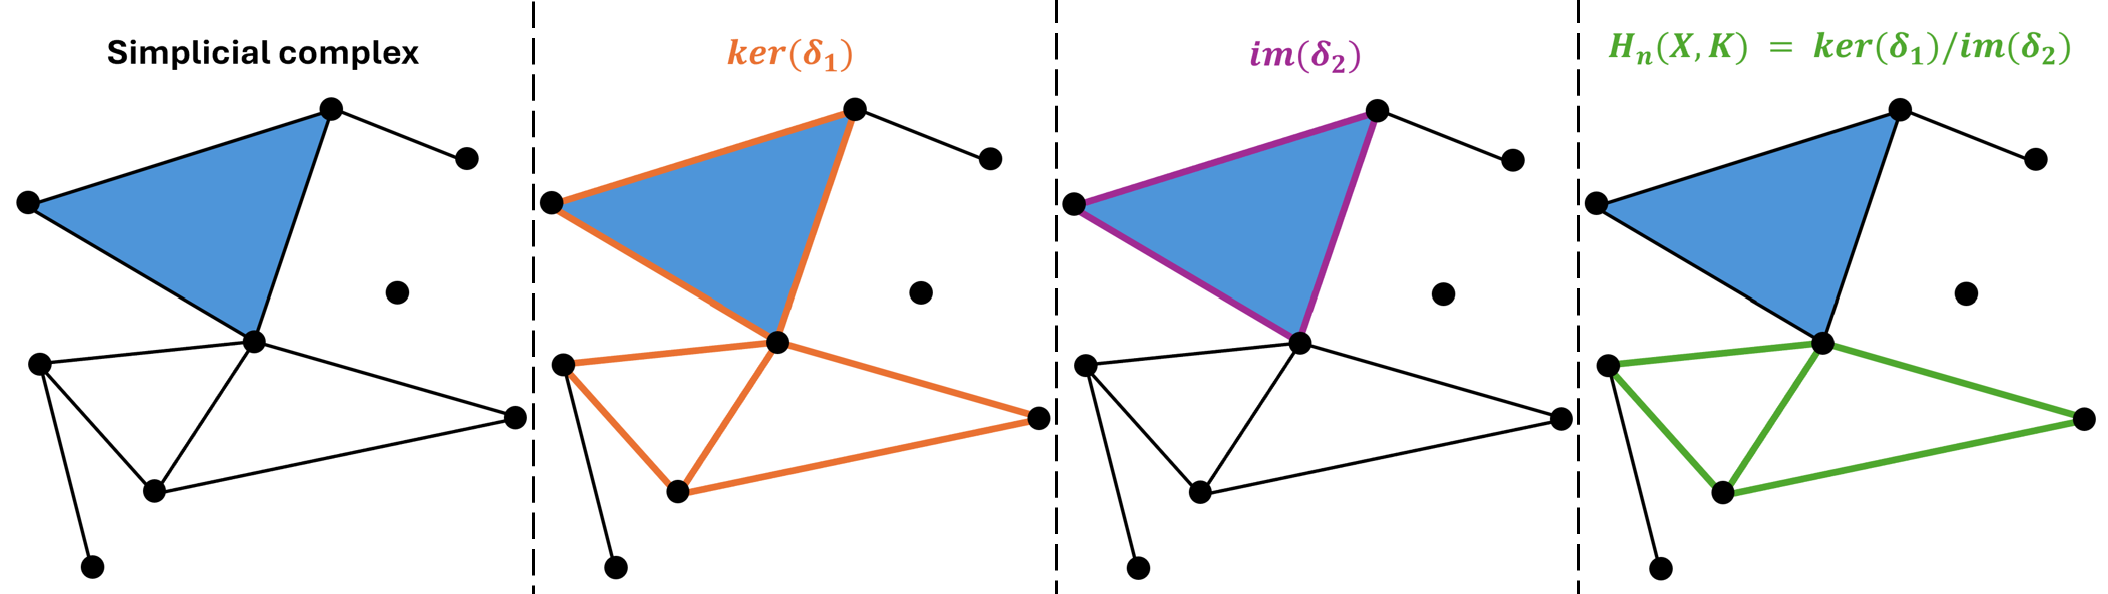
\includegraphics[width=0.99\linewidth]{2nd_homology.png}
    \caption{Example of $2^{nd}$ homology}
    \label{fig:homology}
\end{figure}

If we apply $H_n$ to the Vietoris-Rips filtration, we get one vector space $H_n(VR_t(X),K)$ for each $t$, and the inclusions $VR_{t_1}(X) \subseteq VR_{t_2}(X)$ give the maps between them. So we get a tame vector space parametrized by $[0,\infty)$.

\subsection{Stable rank}
The final step is to transform the parametrized tame vector space (PTVS) into a PCF. A straightforward solution would be to take the rank of the vector space, but this is not stable. To address this, we define the \textbf{stable rank}.

To have a stable map, we need one for which the output doesn't vary too much when the input is slightly modified. First, we need an idea of distance between PTVS to measure how much one varies under a change. Let $V$, $W$ be PTVS,

$d_{\bowtie}(V,W) := \inf \left\{ \epsilon + \tau | V \xrightarrow\psi U \xleftarrow\phi W, \psi \text{ is }\epsilon\text{-eq.}, \phi \text{ is }\tau\text{-eq.} \right\}$

where $V \xrightarrow\psi U$ is an $\epsilon\text{-eq.}$ if $\forall t$,  there is a dotted linear function making the
following diagram commutative:

\[
\begin{tikzcd}[column sep=3cm, row sep=1.5cm]
V_t
    \arrow[r, "V_{t<t+\epsilon}"]
    \arrow[d, "\psi_t"']
&
V_{t+\epsilon}
    \arrow[d, "\psi_{t+\epsilon}"]
\\
W_t
    \arrow[r, "W_{t<t+\epsilon}"']
    \arrow[ur, dotted]
&
W_{t+\epsilon}
\end{tikzcd}
\]

This distance is a metric and we can now define the stable rank as:

\textbf{Definition:}
$\widehat{rank}\,V(t) := \min\left\{ rank(W) | d_{\bowtie}(V,W)\leq t \right\}$

\subsection{Barcodes and how to compute the stable rank}
\label{sec:barcode}
A tame vector space can be described by its \textbf{barcode}: a list of intervals $[b,d)$. Each interval is a homological feature (a connected component for $H_0$, a hole for $H_1$) that is born at scale $b$ and dies at scale $d$. Long bars are features that persist for a long time. Short bars are often just noise.

With the distance $d_{\bowtie}$ that we use, the stable rank can be read directly from the barcode:
\[
    \widehat{rank}\,V(t) = \#\{\text{bars } [b,d) \text{ such that } d-b > t\}.
\]
In words, the stable rank at $t$ counts the bars that are longer than $t$. It starts at the number of bars and decreases to 0. This is the formula we use in practice.

To compare two stable ranks $f$ and $g$, we use the $L^1$ distance:
\[
    d(f,g) = \int_0^\infty |f(t) - g(t)|\, dt .
\]
Since stable ranks are PCFs, this integral is a finite sum and it is easy to compute. We can also take the mean of several stable ranks, point by point. This gives the \textbf{average stable rank} of a group of samples.


\section{Methods}
\label{sec:methods}

Our pipeline is the following:
\begin{center}
    spike train $\rightarrow$ point cloud $\rightarrow$ Vietoris-Rips $\rightarrow$ barcodes $H_0$, $H_1$ $\rightarrow$ stable ranks $\rightarrow$ $L^1$ distances $\rightarrow$ which neuron?
\end{center}
For each trial, we build a point cloud from its spikes and compute the barcodes of its Vietoris-Rips filtration in degrees 0 and 1. We remove the infinite bar of $H_0$, so that every stable rank goes to 0. Each barcode is turned into its stable rank, and two trials are compared with the $L^1$ distance between their stable ranks. Finally, we check if the closest trials come from the same neuron.

\subsection{Selection of the data}
We do not use all 850 neurons. We draw 40 neurons at random among the neurons that fire at least 1 Hz on average, and we keep their first 30 trials. This gives $40 \times 30 = 1200$ spike trains of 10 seconds. If we guess the neuron at random, we are right with probability $1/40 = 2.5\%$. This is the \textbf{chance level}.

To be sure that our results do not depend on a lucky choice of neurons, we repeat everything for 5 different random draws of 40 neurons. We give the mean and the standard deviation over these 5 draws.

\subsection{From a spike train to a point cloud}
There is no unique way to transform a spike train into a point cloud. We use two simple ones.

\subsubsection{Spike times on a line}
The simplest point cloud is the set of spike times $\{t_1, \dots, t_n\} \subset \mathbb{R}$, with the distance $d(t_i,t_j)=|t_i-t_j|$.

For points on a line, the $H_0$ barcode is very easy to understand. At scale $t$, two neighbouring spikes are connected if their distance is at most $t$, that is if their ISI is at most $t$. So each connected component dies when it merges with its neighbour, at $t = \text{ISI}$. The $n$ spikes give $n-1$ bars:
\[
    H_0 \text{ barcode} = \big\{ [0, \text{ISI}_1), [0, \text{ISI}_2), \dots, [0,\text{ISI}_{n-1}) \big\}.
\]
The stable rank at $t$ is then the number of ISIs that are longer than $t$. This is the first procedure of Section~\ref{sec:math} (single linkage on the line). We also checked numerically that the bars we obtain are exactly the ISIs. An example is shown in Figure~\ref{fig:line_example}. We call this method \textbf{LINE}.

\begin{figure}[H]
    \centering
    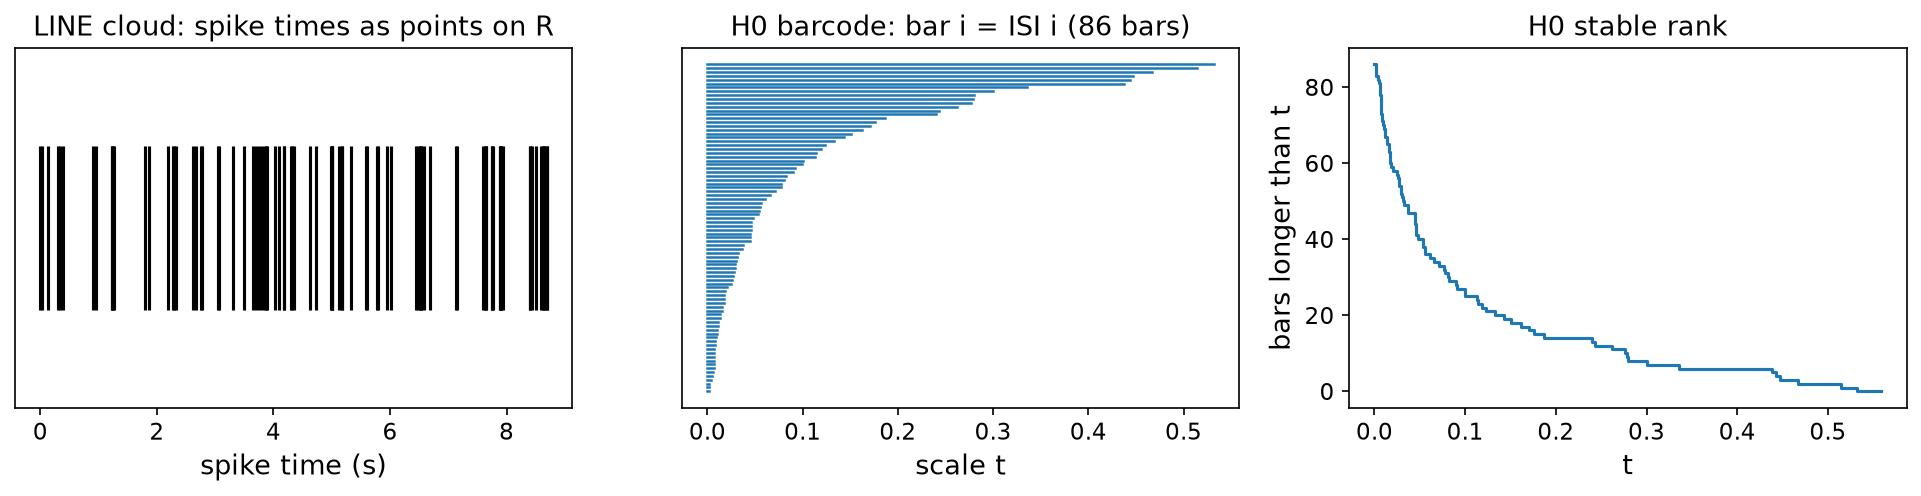
\includegraphics[width=\linewidth]{sr_line_example.png}
    \caption{LINE method for one trial. Left: the spike times. Middle: the $H_0$ barcode, with one bar per ISI. Right: the stable rank, the number of bars longer than $t$.}
    \label{fig:line_example}
\end{figure}

\subsubsection{Delay embedding of the ISIs}
The LINE cloud only sees the lengths of the ISIs, not their order. To also see which ISI follows which, we build a point cloud in $\mathbb{R}^2$ with one point for each pair of consecutive ISIs:
\[
    p_i = \big(\log_{10}\text{ISI}_i,\ \log_{10}\text{ISI}_{i+1}\big), \qquad i = 1,\dots,n-2 .
\]
This is called a \textbf{delay embedding}. A burst (two short ISIs) gives a point in the bottom left corner, a pause after a burst gives a point in the bottom right corner, and so on. We use the logarithm because the ISIs go from 1 ms to several seconds: on a linear scale, all the short ISIs would be squeezed into one point. If a trial has less than 2 ISIs, we use a single point, which has an empty barcode and a stable rank equal to 0. We compute the $H_0$ and $H_1$ barcodes of this cloud with the Euclidean distance. We call this method \textbf{DELAY}.

Figure~\ref{fig:clouds} shows the delay clouds of three neurons. The clouds look different: they have different positions, densities and clusters. Figure~\ref{fig:delay_example} shows the barcodes and the stable ranks of one trial.

\begin{figure}[H]
    \centering
    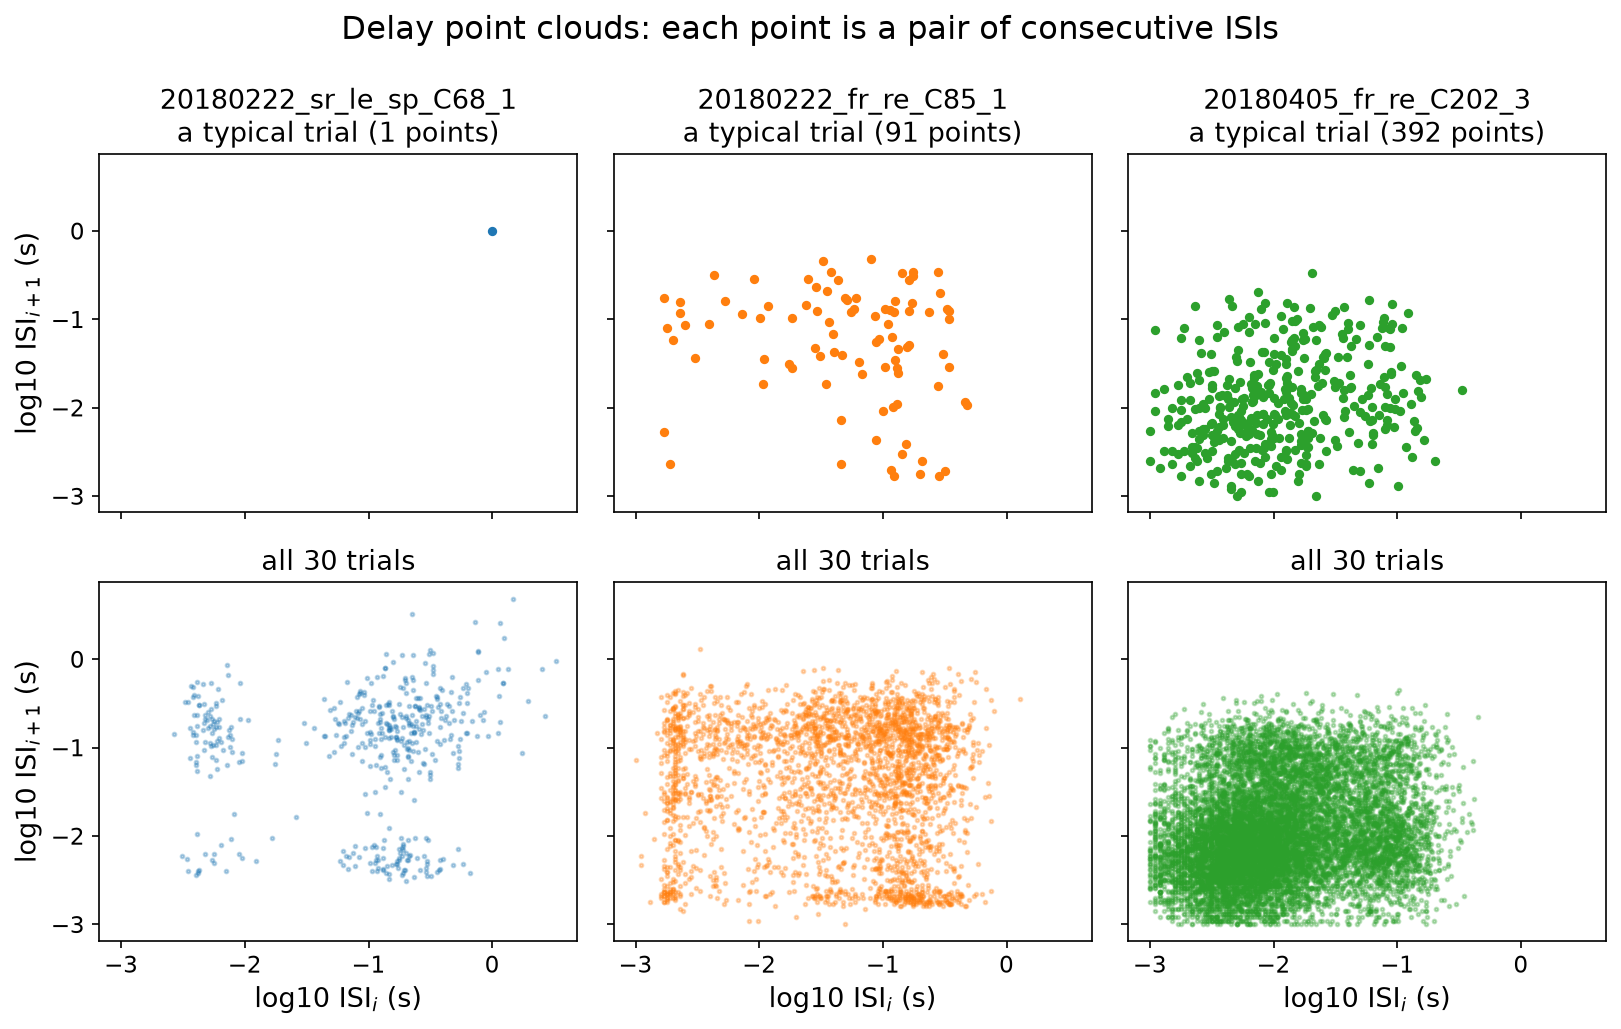
\includegraphics[width=0.85\linewidth]{explore_delay_clouds.png}
    \caption{Delay clouds of three neurons. Top: one typical trial. Bottom: all 30 trials together.}
    \label{fig:clouds}
\end{figure}

\begin{figure}[H]
    \centering
    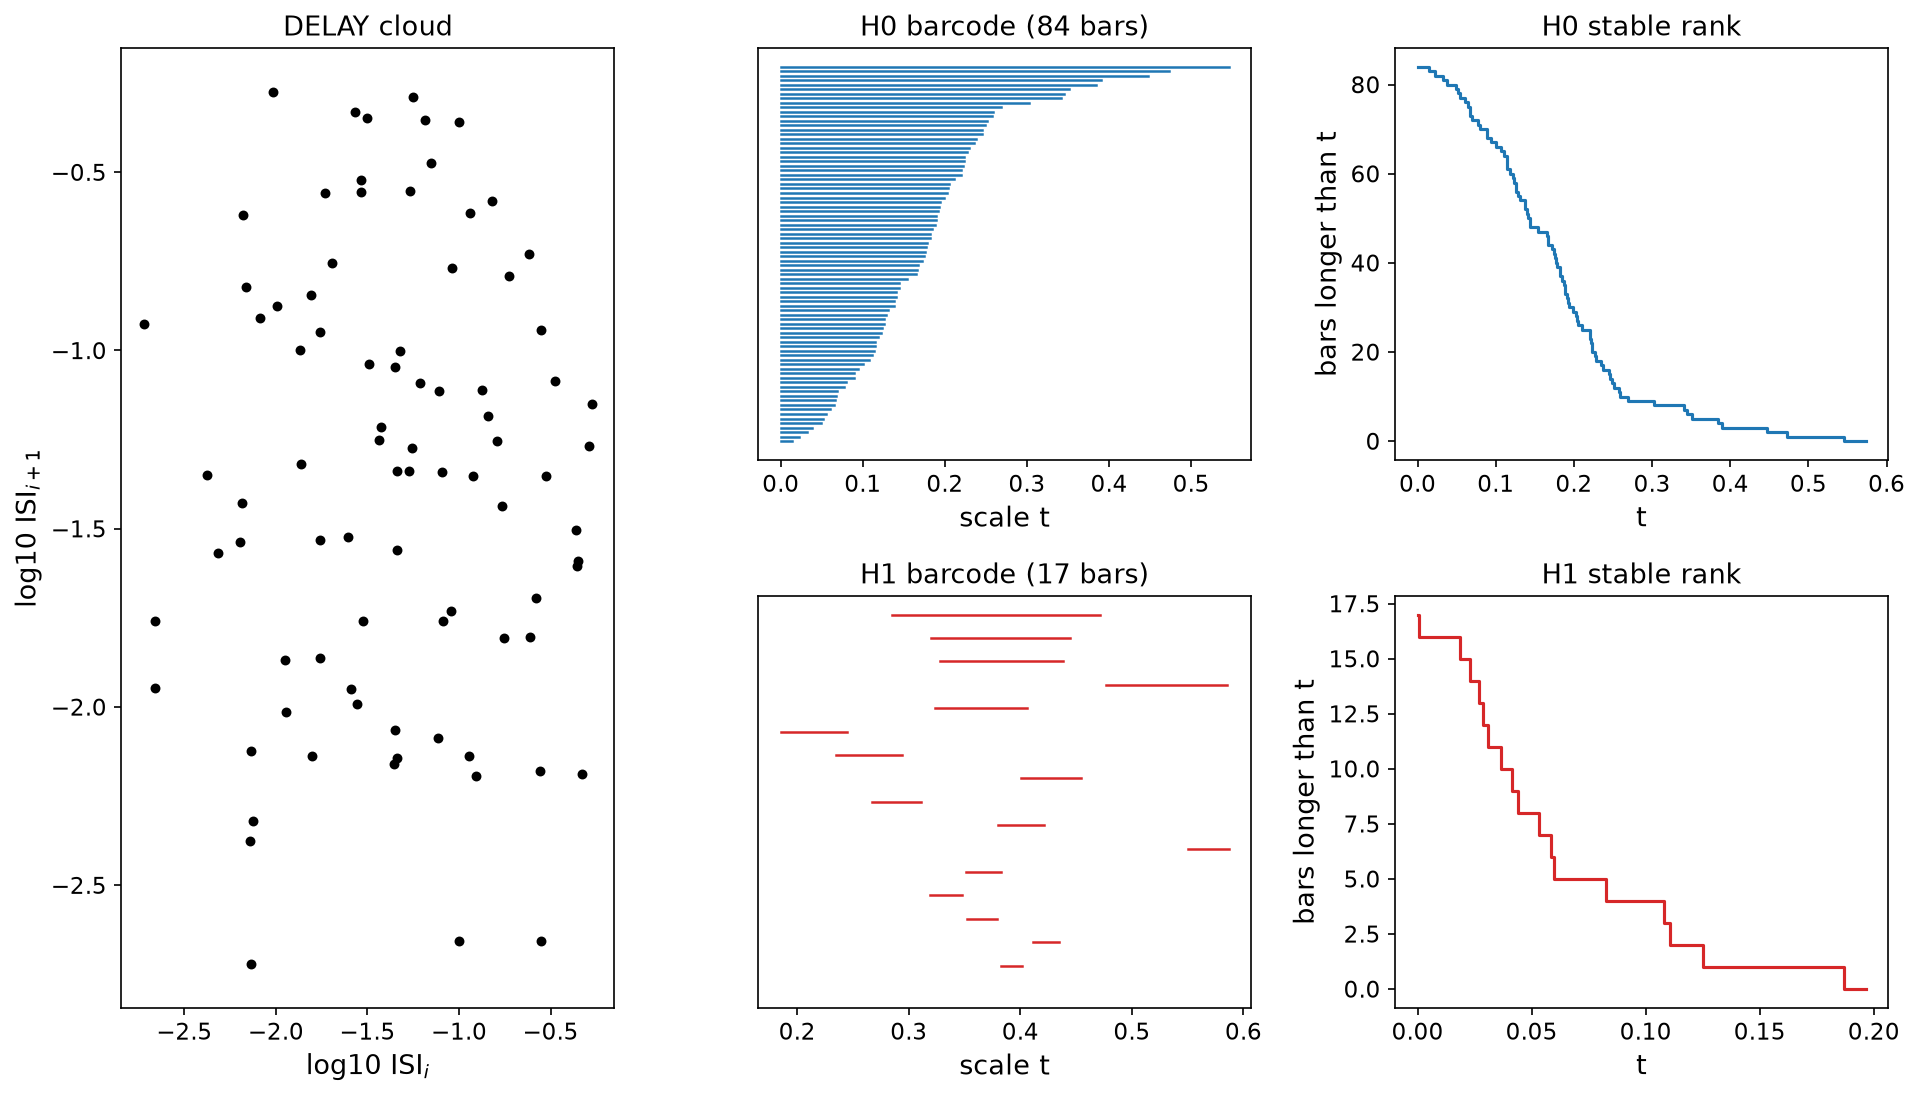
\includegraphics[width=\linewidth]{sr_delay_example.png}
    \caption{DELAY method for one trial: the point cloud, the $H_0$ and $H_1$ barcodes, and their stable ranks.}
    \label{fig:delay_example}
\end{figure}

\subsection{Distances between trials}
Two trials are compared with the $L^1$ distance between their stable ranks (Section~\ref{sec:barcode}). For the DELAY method we have two stable ranks per trial ($H_0$ and $H_1$). The $H_0$ distances are much bigger than the $H_1$ distances, because there are many more $H_0$ bars. If we simply added them, $H_1$ would have almost no effect. So we first divide each distance matrix by its median, and then we add them:
\[
    d_{H_0+H_1} = \frac{d_{H_0}}{\text{median}(d_{H_0})} + \frac{d_{H_1}}{\text{median}(d_{H_1})}.
\]

\subsection{Identifying the neuron}
We use two simple classification rules. We evaluate them with \textbf{leave-one-out cross-validation}. This is a train/test split where the test set is a single trial. Each trial is taken out of the data in turn and becomes the test trial. All the other trials form the training set, and we know their neurons. We classify the test trial using only the training set, and then we put it back and take the next trial.
\begin{itemize}
    \item \textbf{1-nearest neighbour (1-NN):} we look for the training trial that is closest to the test trial. If it comes from the same neuron, the answer is correct.
    \item \textbf{Nearest mean:} for each neuron, we compute the average stable rank of its training trials. Then we give the test trial to the neuron with the closest average stable rank.
\end{itemize}
The neuron of the test trial is never used to classify it: it is only used at the end, to check if the answer is correct. Since the test trial is not in the training set, it is not part of any average. The score of a method is the percentage of test trials that are given to the right neuron.

We chose leave-one-out instead of a split into two halves, because every neuron has only 30 trials. With leave-one-out, the averages are computed from 29 trials instead of 15, and every trial is used once as a test trial.

\subsection{Baselines and control}
To know if topology really helps, we compare with two methods that do not use topology:
\begin{itemize}
    \item \textbf{Firing rate:} we only use the number of spikes in the trial. The distance between two trials is the difference of their firing rates. This tells us how much we can do with the rate alone.
    \item \textbf{ISI histogram:} we compute the histogram of $\log_{10}$ ISI (40 bins from 1 ms to 10 s) and use the $L^1$ distance between histograms. It uses the same information as the LINE method (the set of ISIs), but without topology.
\end{itemize}

We also use a \textbf{control} for the DELAY method. Before building the cloud, we shuffle the ISIs of each trial in a random order. The ISIs are the same, so the distribution of the ISIs does not change, but their order is destroyed. If the DELAY method and its control give the same score, it means that the delay cloud only uses the distribution of the ISIs, and not their order.

Finally, as a sanity check, we gave random labels to the trials. The 1-NN score then drops to 2.6\%, which is the chance level, as expected.

We also study the effect of the length of the samples. We glue 2 or 3 consecutive trials of the same neuron together, which gives samples of 20 or 30 seconds (and 15 or 10 samples per neuron).


\section{Results}
\label{sec:results}

\subsection{Average stable ranks}
Figure~\ref{fig:mean_sr} shows the average stable rank of five neurons, with one standard deviation around it. For some neurons the bands are clearly separated, for example the green neuron, which has fewer bars in all three panels. For other neurons the bands overlap a lot. So we expect that some neurons will be easy to recognise, and others will be confused with each other.

\begin{figure}[H]
    \centering
    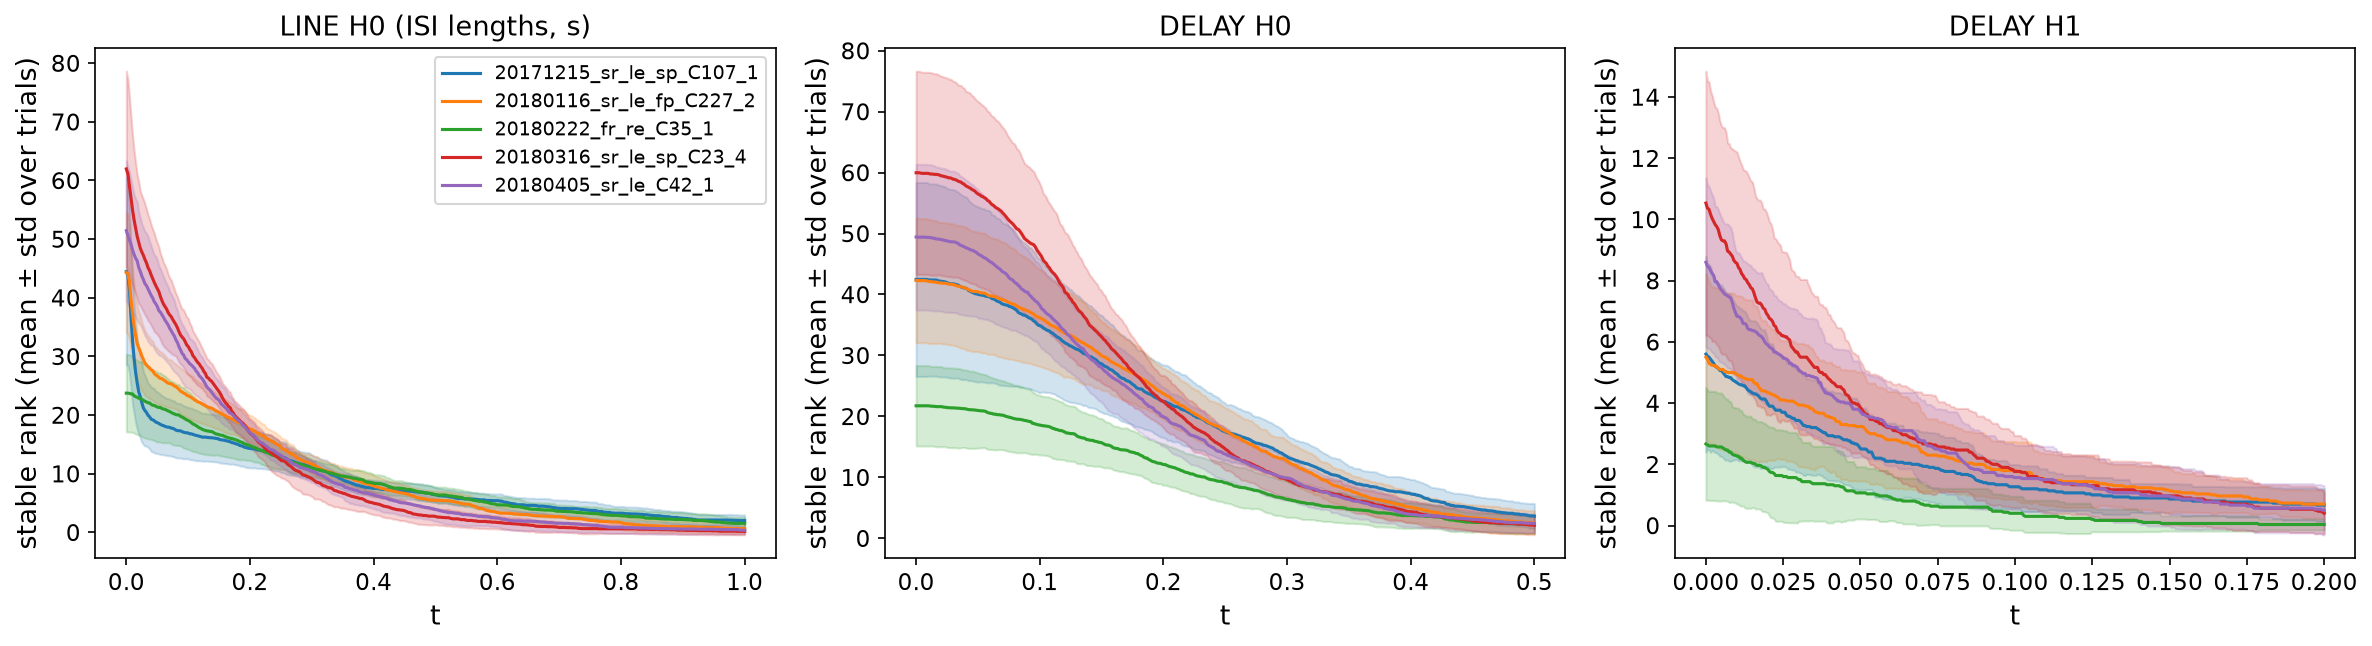
\includegraphics[width=\linewidth]{sr_mean_per_neuron.png}
    \caption{Average stable rank $\pm$ one standard deviation over the 30 trials, for five neurons. Left: LINE $H_0$. Middle: DELAY $H_0$. Right: DELAY $H_1$.}
    \label{fig:mean_sr}
\end{figure}

Figure~\ref{fig:distmat} shows the distances between all the trials of 10 neurons. The trials are sorted by neuron, so the squares on the diagonal contain the distances between trials of the same neuron. These squares are lighter (smaller distances) than the rest of their row for most neurons. This means that the trials of the same neuron are indeed close to each other.

\begin{figure}[H]
    \centering
    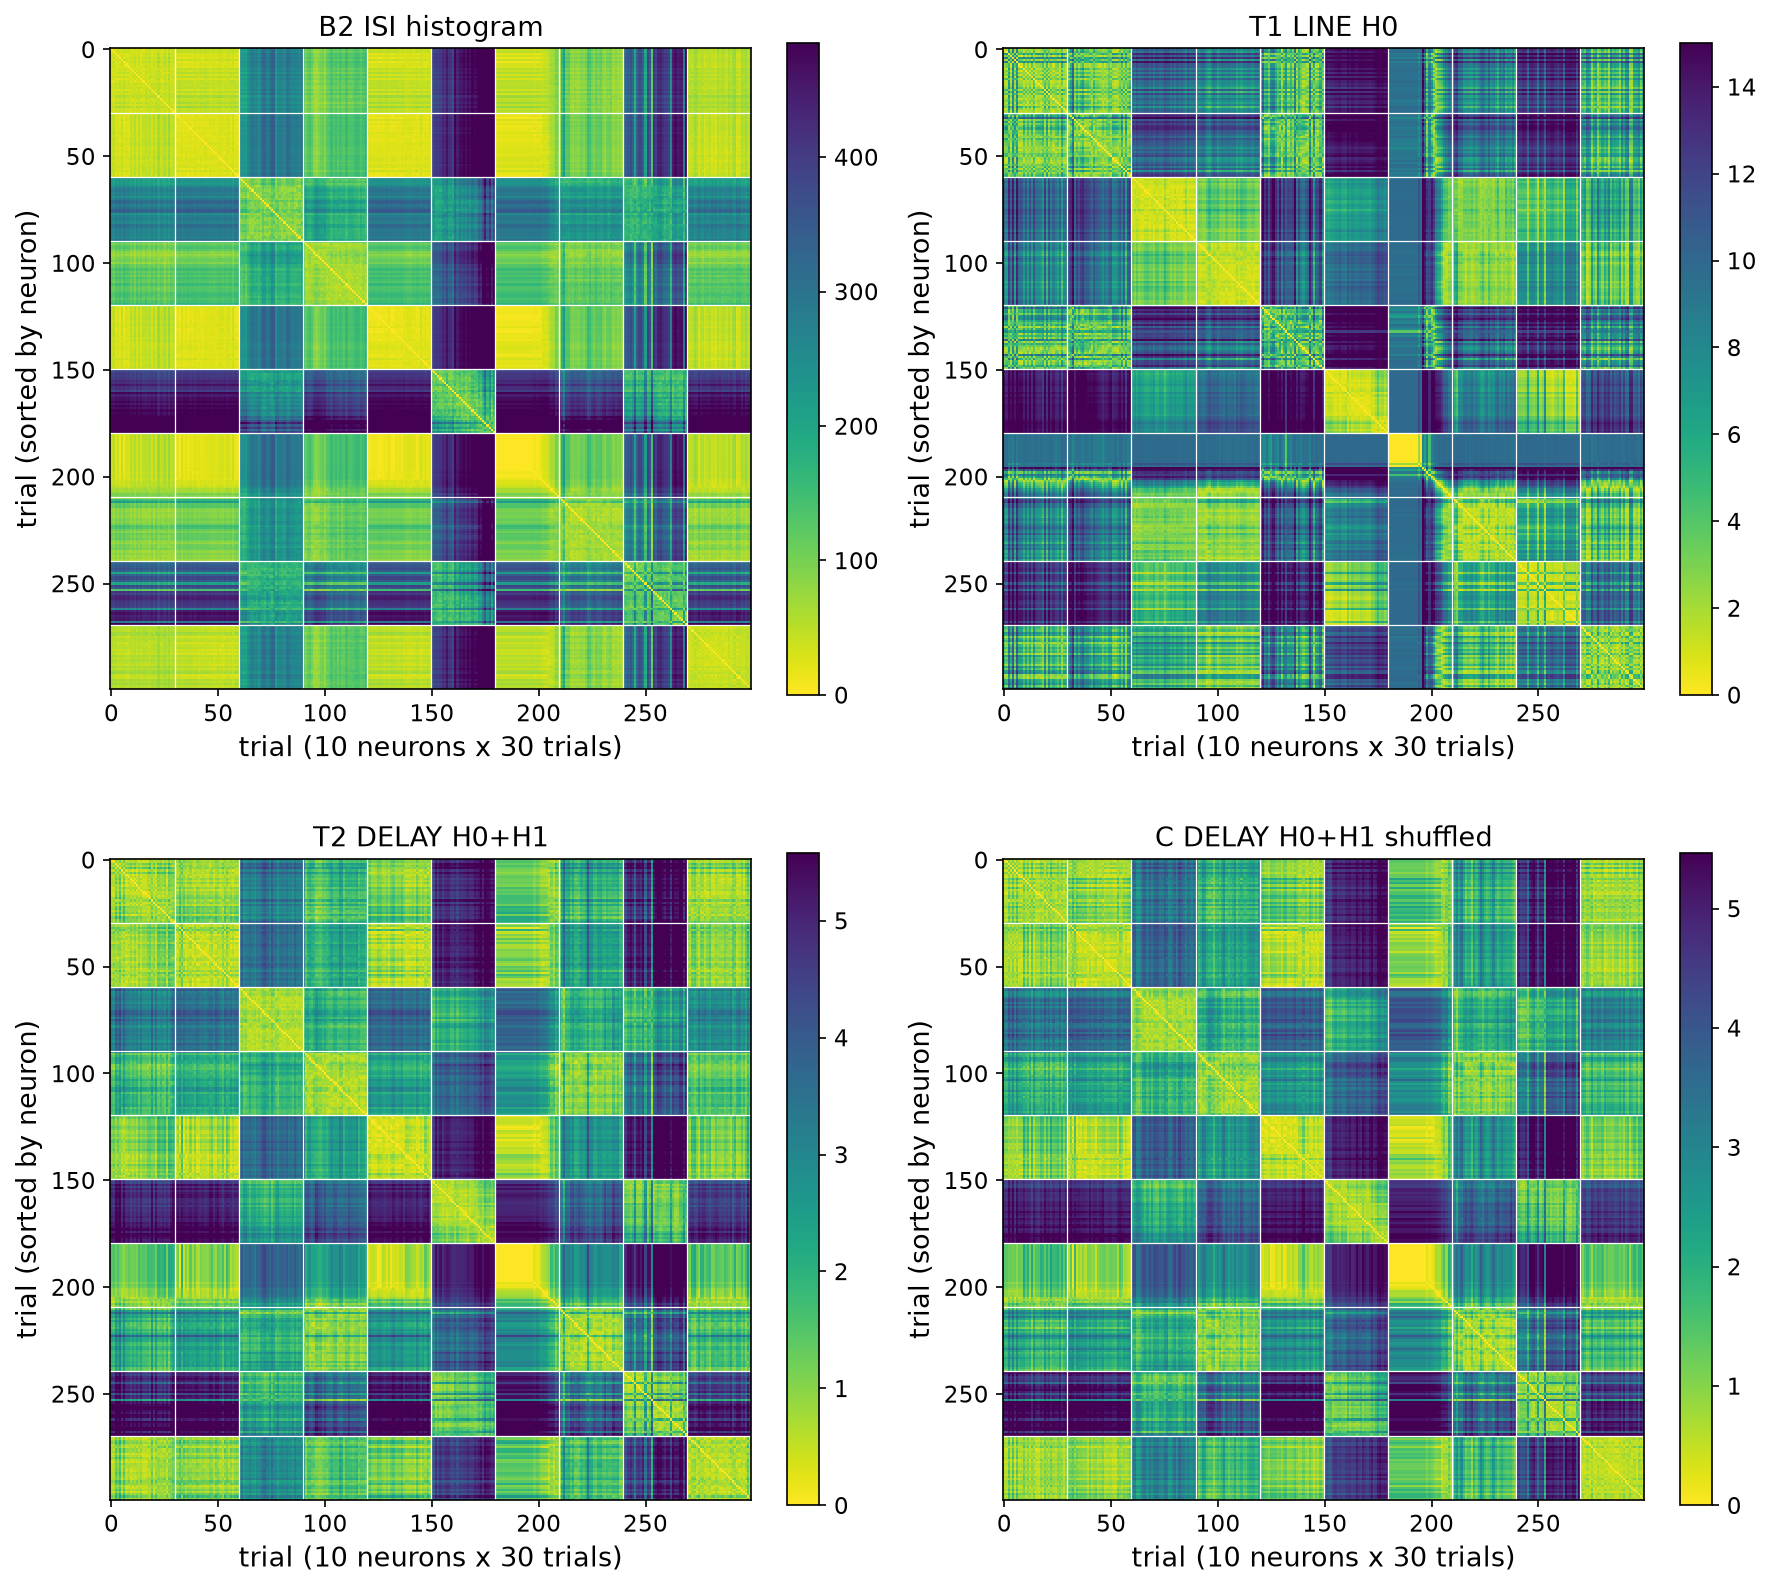
\includegraphics[width=0.8\linewidth]{id_distance_matrix.png}
    \caption{Distances between the 300 trials of 10 neurons, sorted by neuron (the white lines separate the neurons). Light colour = small distance.}
    \label{fig:distmat}
\end{figure}

\subsection{Identification scores}
Table~\ref{tab:scores} and Figure~\ref{fig:scores} give the scores of all the methods for samples of 10 seconds.

\begin{table}[H]
    \centering
    \begin{tabular}{lcc}
        \toprule
        Method & 1-NN (\%) & Nearest mean (\%) \\
        \midrule
        Firing rate (no topology) & $13.2 \pm 2.5$ & $16.0 \pm 3.0$ \\
        ISI histogram (no topology) & $38.1 \pm 7.4$ & $42.1 \pm 5.3$ \\
        \midrule
        LINE $H_0$ & $32.1 \pm 5.3$ & $31.2 \pm 3.6$ \\
        DELAY $H_0$ & $27.9 \pm 6.2$ & $29.0 \pm 4.6$ \\
        DELAY $H_1$ & $13.7 \pm 3.6$ & $18.6 \pm 3.5$ \\
        DELAY $H_0+H_1$ & $26.0 \pm 5.8$ & $27.3 \pm 4.9$ \\
        \midrule
        DELAY $H_0+H_1$, ISIs shuffled (control) & $24.6 \pm 5.9$ & $27.6 \pm 5.0$ \\
        \bottomrule
    \end{tabular}
    \caption{Percentage of trials given to the right neuron, for 40 neurons and 10 s samples (mean $\pm$ standard deviation over 5 random draws of neurons). Chance level is 2.5\%.}
    \label{tab:scores}
\end{table}

\begin{figure}[H]
    \centering
    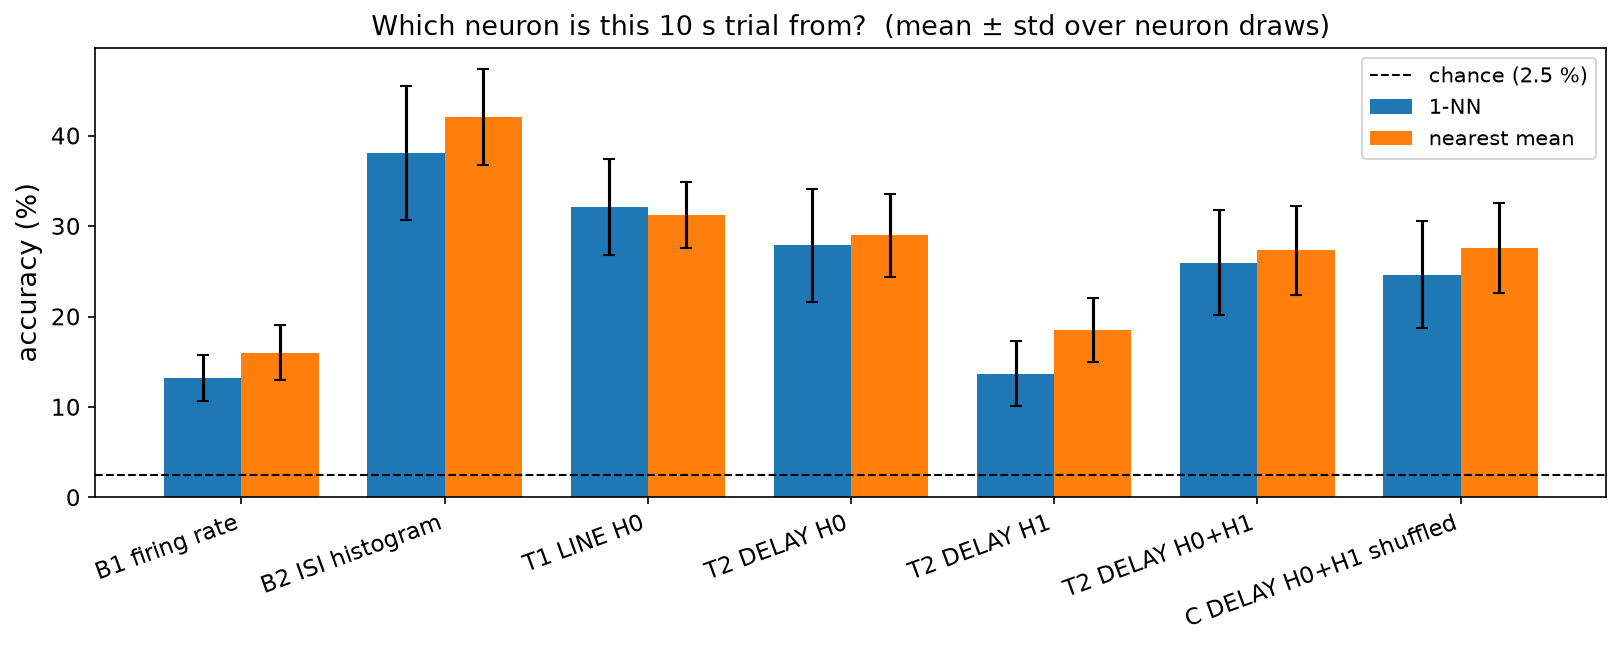
\includegraphics[width=\linewidth]{id_scores.png}
    \caption{Scores of the methods. The dashed line is the chance level.}
    \label{fig:scores}
\end{figure}

We can make the following observations.

\textbf{The stable ranks can identify the neurons.} With the LINE method, about 31\% of the trials are given to the right neuron, against 2.5\% by chance. This is 12 times better than chance. So each neuron does have a signature in its spike trains, and a single trial of 10 seconds is enough to see it.

\textbf{It is not only the firing rate.} The firing rate alone gives 13--16\%. The stable ranks give about twice this score. So they capture \textit{how} the neuron fires, and not only \textit{how much} it fires.

\textbf{The order of the ISIs does not help.} The DELAY method with $H_0$ and $H_1$ (27.3\%) gives the same score as its control with shuffled ISIs (27.6\%). This means that the topology of the delay cloud is mostly decided by which ISIs occur, and not by their order. The delay cloud does not do better than the simpler LINE method.

\textbf{$H_1$ is weak.} $H_1$ alone gives only 14--19\%, and adding it to $H_0$ makes the score a little lower (29.0\% $\rightarrow$ 27.3\%). Our clouds are small (between about 10 and 150 points for 10 seconds), so they do not have meaningful holes. Most $H_1$ bars are short, which means they are mostly noise.

\textbf{The ISI histogram is the best method.} The simple histogram of $\log_{10}$ ISI gives 42\%, more than all the topological methods. We think that the main reason is the scale. The histogram uses a logarithmic scale, so short ISIs (bursts) count as much as long ISIs. The $L^1$ distance between LINE stable ranks is an integral over $t$ on a linear scale, so it is dominated by the long ISIs. To check this, we computed the histogram with a linear scale instead: it gives 24--32\% (on 3 draws), about the same as the LINE method. We also tried to give the logarithm of the ISIs to the LINE method, but it did not improve the score (23--31\%).

\subsection{Effect of the sample length}
Figure~\ref{fig:length} shows the nearest-mean score when the samples are longer. All the methods except the firing rate get better when we have more data: from 10 to 30 seconds, they gain between 6 and 9 points (for example, LINE goes from 31.2\% to 37.7\%, and the histogram from 42.1\% to 51.2\%). So the signatures are real, but they are noisy in short samples.

\begin{figure}[H]
    \centering
    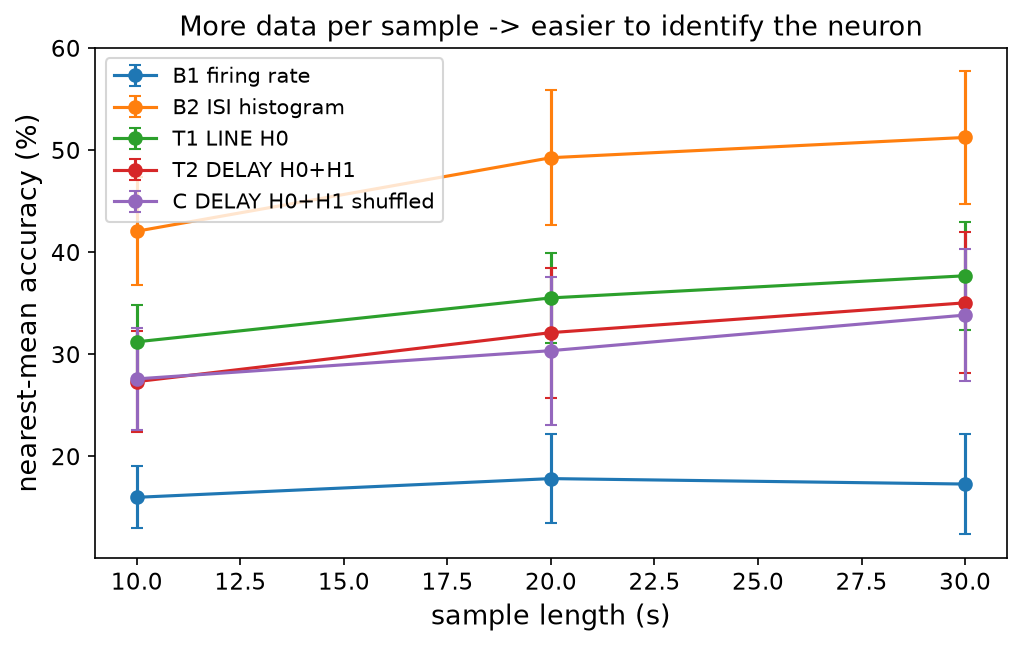
\includegraphics[width=0.7\linewidth]{id_sample_length.png}
    \caption{Nearest-mean score against the length of the samples (mean $\pm$ standard deviation over 5 draws).}
    \label{fig:length}
\end{figure}

\subsection{Limitations}
Our study has some limitations:
\begin{itemize}
    \item All the trials show the same movie. So the signature that we find could partly be ``the response to this movie'' and not only a property of the neuron.
    \item The firing rate changes during the recording, and some neurons are almost silent in the first trials. This makes the trials of the same neuron less similar.
    \item The samples are short (10 seconds), and we saw that longer samples give better scores.
    \item We only used neurons that fire at least 1 Hz, and 40 neurons at a time.
\end{itemize}


\section{Conclusion}
\label{sec:conclusion}
In this project, we asked if a single spike train can tell which neuron it comes from. We transformed each spike train into a point cloud, computed its Vietoris-Rips barcodes and its stable ranks, and compared the stable ranks with the $L^1$ distance.

The answer is yes, partly. From one trial of 10 seconds, the stable ranks find the right neuron among 40 in about 30\% of the cases, which is 12 times better than chance and twice better than the firing rate alone. The simplest method, the $H_0$ of the spike times on a line, works best among the topological methods. Its bars are exactly the ISIs. The delay embedding and $H_1$ did not add information: the delay cloud gives the same result when we shuffle the order of the ISIs.

However, a simple histogram of the logarithm of the ISIs does better than our topological methods (42\%). In our setting, the information that the stable ranks use is the distribution of the ISIs, and the histogram on a logarithmic scale captures it better. A possible improvement would be to compare the stable ranks on a logarithmic scale of $t$. Another direction is to use the timing of the spikes in the movie (the vertical lines of Figure~\ref{fig:raster}), which our methods do not use.

\end{document}
